\chapter{Dodatkowe produkty pracy}
W trakcie tworzenia niniejszej pracy powstało także kilka produktów ubocznych, które zdaniem autora mają szanse zostać popularnymi wtyczkami do szkieletu aplikacji Vaadin oraz o których warto wspomnieć. Każda z tych wtyczek używa adnotacji zaszytych bezpośrednio w klasie obiektu, na których operują.

\section{Przykładowa klasa modelu danych}
Implementacja systemu opierała się przede wszystkim przy użyciu komponentów wymienionych w tym rozdziale. Każdy z nich korzysta ze stworzonych od nowa adnotacji, którymi opatrzone są definicje klas:
\begin{itemize}
\item ColumnHeader - definiuje nagłówek oraz kolejność przedstawiania właściwości obiektu w komponencie CRUDTable
\item EditField - opisuje sposób wyświetlania pola edycji odpowiedzialnego za wypełnienie pola z którym jest związane (kolejność wyświetlenia oraz opis, a także dodatkowa informacja używana w implementacji - obiekt klasy będący typem generycznym zbioru, będącego opisywanym polem.
\item ForeignFieldLabel - umożliwia konfiguracje sposobu wyświetlania klasy obiektu w komórce tabeli (CRUDTable) jak i polu słownikowym (ForeignField).
\end{itemize}

Poniżej została przedstawiona uproszczona standardowa klasa zawierająca konfiguracje z użyciem adnotacji używana przez wymienione w tym rozdziale komponenty. 
\begin{lstlisting}
@Entity
@Table(name = "figure_specifications")
@ForeignFieldLabel(pattern = "id")
public class FigureSpecification
{
	@Id
	@GeneratedValue
	@Column(name = "figure_specification_id")
	private Long id;
\end{lstlisting}
\newpage
\begin{lstlisting}
	@Column(name = "figure_specification_profile")
	@ColumnHeader(value = "Profil", order = 3)
	@EditField(label = "Profil", order = 3)
	@NotNull
	private Boolean profile = false;

	@Column(name = "figure_specification_projection")
	@ColumnHeader(value = "Rzut", order = 2)
	@EditField(label = "Rzut", order = 2)
	@NotNull
	private Boolean projection = false;

	@JoinColumn(name = "figure_id")
	@NotNull(message = "Rysunek nie moze byc pusty")
	@ManyToOne(optional = false)
	private Figure figure;

	@JoinColumn(name = "object_id")
	@ColumnHeader(value = "Obiekt", order = 1)
	@EditField(label = "Obiekt", order = 1)
	@NotNull(message = "Obiekt nie moze byc pusty")
	@ManyToOne(optional = false)
	private ArchObject archObject;
	...
	(gettery i settery)
}
\end{lstlisting}
Jak widać, w powyższej klasie zostały użyte trzy typy adnotacji:
\begin{itemize}
\item javax.persistence - odpowiedzialne za mapowanie relacyjno-obiektowe wewnątrz systemu
\item javax.validation - odpowiedzialne za walidacje wprowadzonych wartości
\item dedykowane dla stworzonych komponentów
\end{itemize}
Jak dalej zostanie opisane w tym rozdziale, każdy z wyżej wymienionych rodzajów jest wykorzystywany przez niżej opisane komponenty.

\newpage
Warto zwrócić także uwagę na adnotację @ForeignFieldLabel, zawierającą definicje sposobu wyświetlania obiektu POJO w poniższych komponentach. Składnia wyrażenia zawartego w adnotacji pozwala wyświetlać zarówno pojedyńcze pole (wartość "nazwa\_pola" lub "\$nazwa\_pola\$") lub kombinacje jednego bądź większej ilości pól ze statycznym ciągiem znaków (np. "Pan: \$imie\$ \$nazwisko\$", nazwy zmiennych zawierają sie między znakami "\$"). Jedynym warunkiem poprawnego wyświetlenia napisu odpowiadającego wartościom obiektu jest konieczność implementowania przez użyte pola metody toString().

\section{CRUDTable}
CRUDTable to komponent, który wyświetla listę obiektów wykorzystując wtyczkę FilterTable opartą na komponencie CustomTable wzbogaconą o standardowe przyciski generujące akcje związane z przetwarzaniem danych tabelarycznych, tzn. dodawania, edytowania i usuwania wierszy. Dodatkowo, zaimplementowana jest funkcjonalność z użyciem wtyczki ContextMenu, która zawiera domyślnie także akcje związane z przetwarzaniem zbioru danych.

\begin{figure} [H]
    \begin{center}
	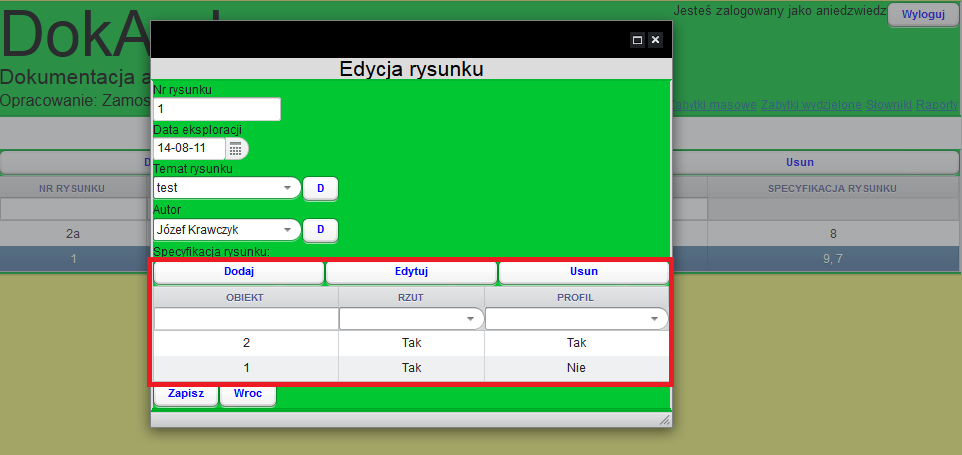
\includegraphics[scale=.6]{img/crudTable.png}
	\caption{Komponent CRUDTable (zaznaczony na czerwono)}
	\label{crudTable}
    \end{center}
\end{figure}

Nic nie stoi na przeszkodzie, aby rozszerzać funkcjonalność komponentu CRUDTable. Istnieją metody pozwalające modyfikować listę przycisków znajdujących się nad tabelą, można także dodawać pozycje widoczne w menu kontekstowym.

\newpage
Dzięki wykorzystaniu komponentu FilterTable istnieje możliwość filtrowania wierszy ze względu na wartości przechowywane w konkretnych polach. Istnieje możliwość zawężenia wyświetlanych rekordów zarówno po wartościach liczbowych jak i wartościach tekstowych, a nawet takich, które odwołują się do innych obiektów dziedziny problemu (czyli będących kluczem obcym).

Najważniejszą jednak funkcjonalnością jest sterowanie wyglądem treści przedstawianej przez komponent za pomocą adnotacji. Dopisując adnotacje @ColumnHeader do pola obiektu POJO definiuje się tak naprawde wygląd tabelki wyświetlającej dany obiekt. Atrybut value definiuje nam wartość widoczną w nagłówku kolumny natomiast parametr order decyduje o kolejności wyświetlanych kolumn (są one wyświetlane w kolejności rosnącej). Uwaga! To programista jest odpowiedzialny za poprawne wypełnienie wartości order, w przypadku zdublowania wartości wyświetlona zostanie tylko jedna kolumna.

Warto także dodać, że w kolumnie w sposób sensowny są także wyświetlane inne obiekty niekoniecznie będące typami prostymi w Javie. Aby wyświetlić poprawnie obiekt, wystarczy do deklaracji klasy dodać adnotacje ForeignFieldLabel, która opisuje w jaki sposób wyświetlić wartość w danej komórce tabeli.

Obiekt, który zawiera w sobie komponent CRUDTable powinien implementować interfejs CRUDTableListener, ponieważ sam komponent nie podejmuje żadnych akcji w wyniku zdarzeń wygenerowanych przez użytkownika, a jedynie przekazuje je dalej do nasłuchiwaczy. Obiekt ten jest także odpowiedzialny za wypełnienie komponentu wartościami.

\section{ForeignField}
Kolejnym komponentem, który wg autora może być przydatny w innych projektach jest ForeignField, który implementuje kontrolkę odpowiedzialną za wprowadzenie wartości ze słownika. Kontrolka używa komponentu ze standardowego zestawu komponentów Vaadina - ComboBox oraz przycisku.

\newpage
\begin{figure} [H]
    \begin{center}
	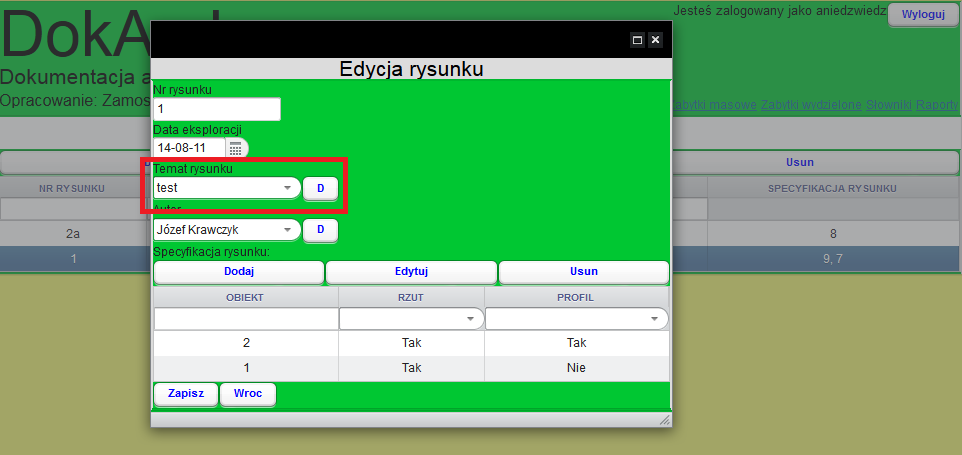
\includegraphics[scale=.6]{img/foreignField.png}
	\caption{Komponent ForeignField (zaznaczony na czerwono)}
	\label{formField}
    \end{center}
\end{figure}

Użycie kontrolki sprowadza się do zdefiniowania wartości wyświetlanej jako wartość obiektu w liście rozwijanej (adnotacja @ForeignFieldLabel) oraz ustawienie listy możliwych wartości. Uwaga! Kontrolka sama w sobie nie podejmuje żadnych akcji po naciśnięciu przycisku. Obiekt, który zawiera w sobie komponent powinien implementować interfejs DictionaryFieldListener i tam zdefiniować zachowanie będące reakcją na naciśnięcie przycisku "D".
\section{DefaultForm}
DefaultForm jest komponentem, który na podstawie adnotacji @EditField zawartych w klasie obiektu tworzy formularz złożony z domyślnych komponentów Vaadina oraz dwóch poprzednio wymienionych: CRUDTable oraz ForeignField. 

\newpage
\begin{figure} [H]
    \begin{center}
	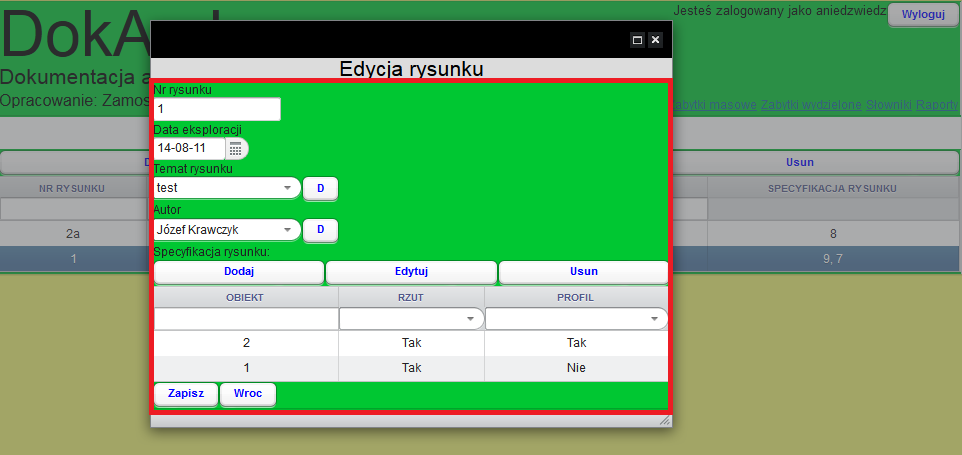
\includegraphics[scale=.6]{img/formField.png}
	\caption{Komponent DefaultForm (zaznaczony na czerwono)}
	\label{defaultForm}
    \end{center}
\end{figure}

Adnotacja @EditField zawiera w sobie informacje na temat kolejności wyświetlania komponentów do edycji kolejnych wartości obiektu (wartość order) oraz wartość etykiety (label), która powinna być wyświetlona przy danym polu. Uwaga! To programista jest odpowiedzialny za poprawne wypełnienie wartości order, w przypadku zdublowania wartości wyświetlona zostanie tylko jedno pole edycji.

Komponent DefaultForm deleguje zadanie tworzenia kontrolek do obiektu-fabryki implementującego interfejs ExtendedFieldGroupFieldFactory (rozszerzającego interfejs Vaadina FieldGroupFieldFactory). W zależności od typu pola obiektu tworzona jest inna kontrolka. Dla standardowych typów takich jak Integer lub String, kontrolki generowane są przez domyślną fabryke Vaadina - FieldGroupFieldFactory. W przypadku wystąpienia przy polu adnotacji javax.persistence odpowiedzialnych za relacje Wiele-Do-* lub Jeden-Do-Wielu generowana jest odpowiednia kontrolka. Jeżeli nad polem znajduje się adnotacja @ManyToOne, generowana jest kontrolka typu ForeignField, natomiast dla adnotacji @OneToMany oraz @ManyToMany, generowany jest komponent CRUDTable.

Aby wypełnić słowniki, należy dostarczyć do komponentu DefaultForm obiekt, który implementuje interfejs DataProvider, ponieważ komponent sam w sobie nie potrafi wypełnić ich wartościami.

\newpage
DefaultForm nie podejmuje także samodzielnie żadnych akcji, a jedynie oddelegowuje je do zarejestrowanych listenerów. Komponent przechwytuje także zdarzenia wygenerowane w zawartych komponentach ForeignField i CRUDTable, czyli jest ich nasłuchiwaczem, jedyne co robi z tymi zdarzeniami to przekazuje je dalej, dlatego istotne jest, aby obiekt zawierający w sobie komponent DefaultForm implementował interfejs FormFieldListener. Dodatkowo, aby przechwytywać zdarzenia związane z przyciskami "Zapisz" oraz "Wróć" należy zarejestrować nasłuchiwacz implementujący interfejs FormListener.

Ważną cechą komponentu DefaultForm, o której należy wspomnieć na koniec, jest walidacja wprowadzonych wartości na podstawie adnotacji javax.validation. Wszystkie standardowe ograniczenia na wartości pól, zgodne z JSR-303 są sprawdzane przed wysłaniem akcji "zapisz" do obiektu nasłuchującego. W przypadku niepowodzenia walidacji, zdarzenie nie jest przekazywane dalej.
\section{Szkielet aplikacji przetwarzania danych biznesowych}
W trakcie tworzenia systemu wspierającego prowadzenie ewidencji zabytków archeologicznych powstał także szkielet aplikacji, który został opisany w rozdziale 5.

% ex: set tabstop=4 shiftwidth=4 softtabstop=4 noexpandtab fileformat=unix filetype=tex spelllang=pl,en spell: